\chapter{HTWG Lab Cloud}

Nachfolgend werden die Ziele, Anwendungsfälle und die eigentliche Implementierung des Projekts erläutert.

Der Quellcode ist öffentlich auf GitHub \cite{git-source} verfügbar. Weitere Entwicklungen finden stets in diesem Repository statt. Etwaige Pull-Request werden gerne angenommen.

\section{Zielsetzung}
Erfahrungsgemäß jeder Student kennt das folgende Problem. Eine Vorlesung wird
besucht, in welcher neue Technologien kennengelernt werden. Folglich werden neue Anwendungen
eingesetzt, die zunächst installiert werden müssen. 
Findet die Vorlesung in einem Laborraum statt, 
so ist die notwendige Software meist schon installiert.
Dabei sind spezielle Anwendungen häufig nicht in allen Laboren vorzufinden. Folglich müsste
eine Vorlesung in einem entsprechenden Raum stattfinden.
Das Installieren der Software ist zudem ein umständlicher Prozess. Ein Dozent muss hierfür
das Rechenzentrum beauftragen, welches dann die notwendige Software installiert.
Folglich wäre es viel einfacher wenn ein Professor die für seine Vorlesung erforderliche Software
eigens zusammenstellen könnte.
Zudem wäre es für einen Studenten wünschenswert, den Zugriff auf die Software einer Vorlesung,
von jedem beliebigen Laborrechner zu erhalten.
Die HTWG Lab Cloud will die so eben beschriebenen Probleme lösen und einen Cloud Dienst zur
Verfügung stellen. Dieser Dienst soll das einfache Erstellen von virtuellen Maschinen für
Vorlesungen zur Verfügung stellen. Die somit erstellten virtuellen Maschinen sollen dann für
einen Studenten über eine entsprechende Remote Verbindung zugreifbar sein.

Die Ziele der HTWG Lab Cloud sind wie folgt definiert:
\begin{itemize}
\item Bereitstellen einer Konfiguration von virtuellen Maschinen für Professoren.
\item Starten von virtuellen Maschinen für die Teilnehmer einer Vorlesung.
\item Ein vom Laborraum unabhängiger Zugriff auf virtuelle Maschinen durch Studenten.
\item Die Nutzung der vorhandenen Authentifizierungsmethoden der Hochschule.
\end{itemize}

Die nachfolgende Abbildung \autoref{overview} soll einen Überblick über 
die vorhandenen Komponenten der HTWG Lab Cloud geben. Ein Professor kann über einen
Webbrowser auf das Dashboard der Cloud zugreifen. Dabei zeigt das Dashboard die Vorlesungen
eines Professors an. Für die Teilnehmer einer Vorlesung kann daraufhin eine virtuelle Maschine
mit einem ausgewählten Image gestartet werden. Dabei stehen dem Professor eine Reihe von Basis
Images bereit, welche er beliebig erweitern kann.
Nachdem die virtuellen Maschinen für die Studenten gestartet wurden, kann auf diese mittels
VNC zugegriffen werden.
Die Details zum eben genannten groben Überblick sind in den nachfolgenden 
Unterkapiteln nachzulesen.

\begin{figure}[H]
	\centering
	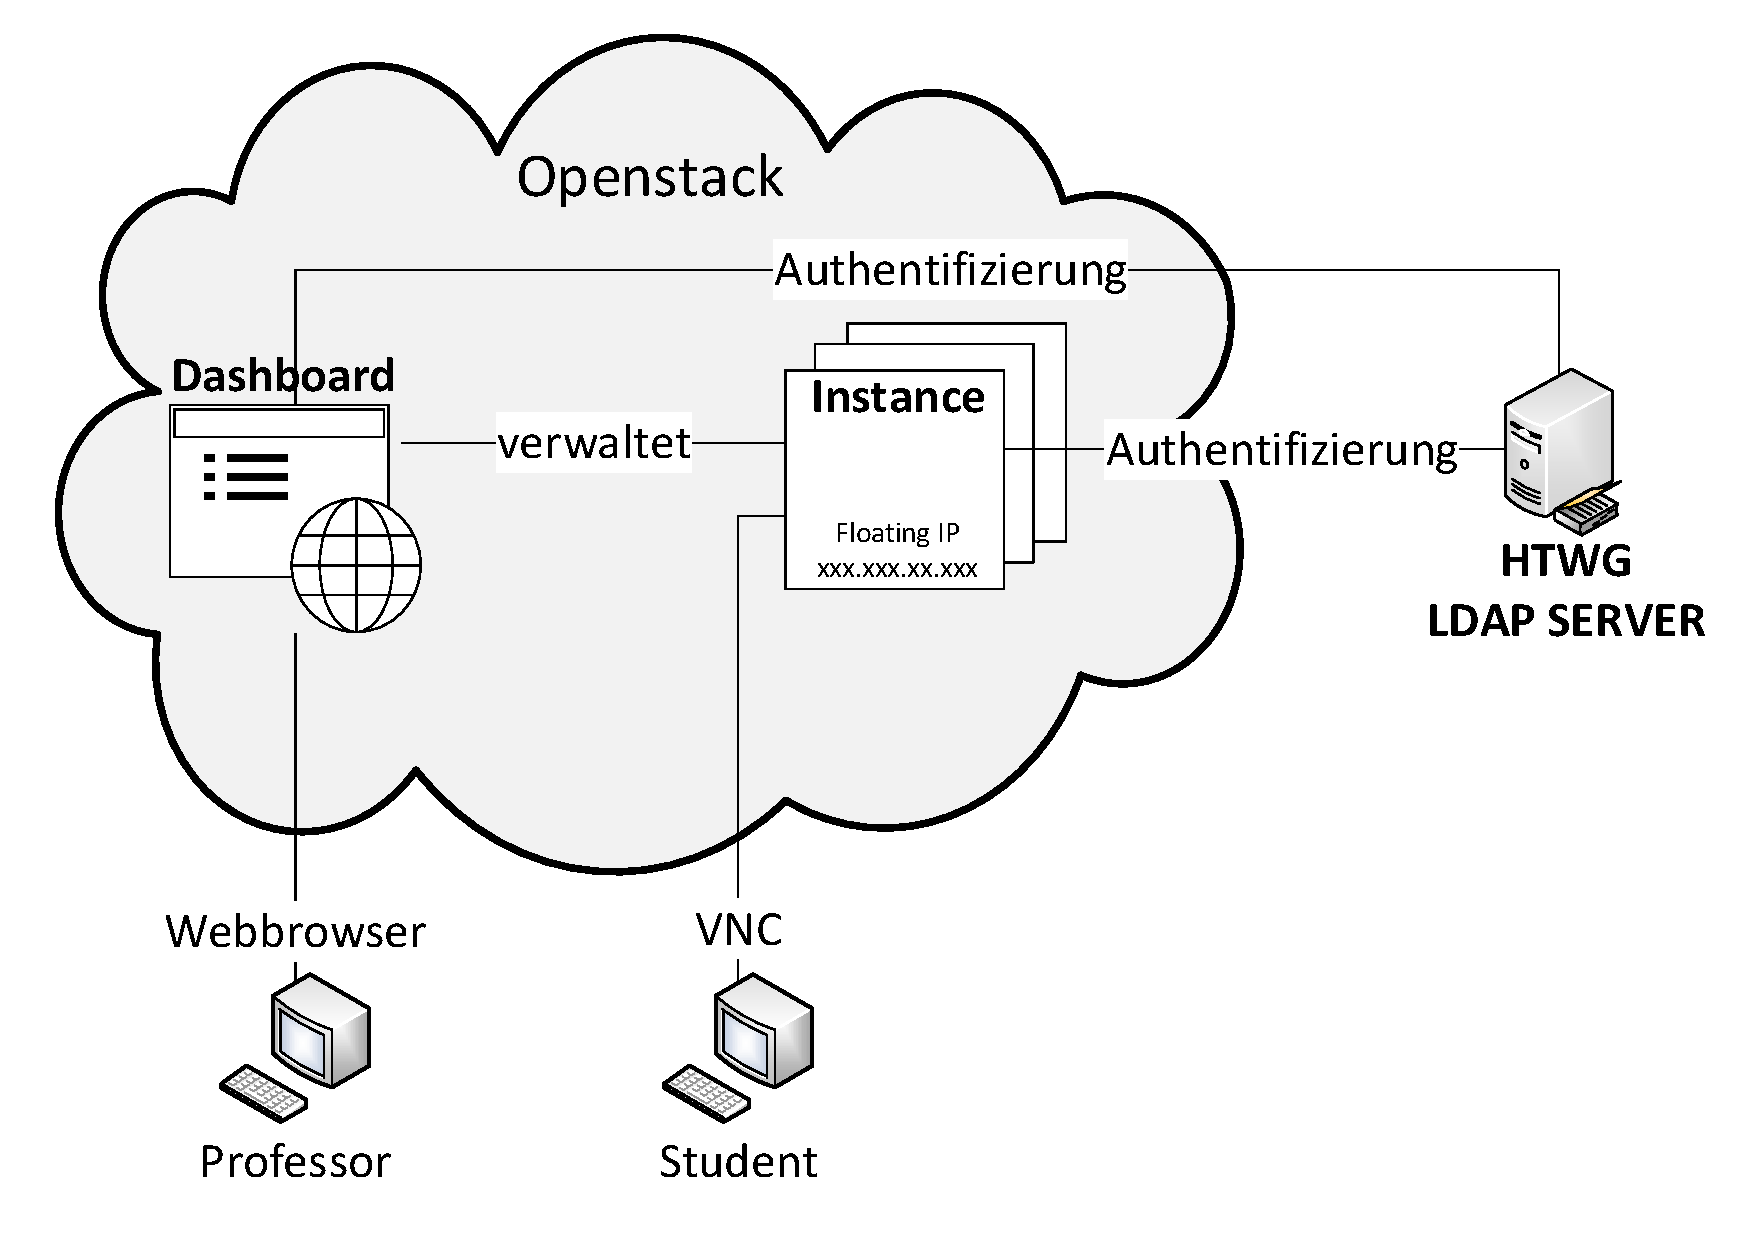
\includegraphics[scale=0.4]{img/overview.pdf}
\caption{Überblick HTWG Lab Cloud}
\label{overview}
\FloatBarrier
\end{figure}

\section{Workflow und Organisation}
In diesem Abschnitt werden die internen Abläufe der HTWG Lab Cloud erläutert. Die folgenden
Vorgänge sind völlig transparent für einen Professor und Studenten und dienen lediglich zum
Verständnis der technischen Umsetzung.
Dabei soll die Kommunikation mit den notwendigen Openstack Komponenten verdeutlicht werden.
Also beispielsweise welche Komponenten für das Starten von virtuellen Maschinen Instanzen 
für eine Vorlesung notwendig sind.
In den nachfolgenden Grafiken wird zur Übersicht auf die Darstellung von
Authentifizierungsschritten verzichtet, wenngleich diese in der Implementierung vorzufinden sind.
Weitere Informationen über die Authentifizierung über LDAP sind in den nachfolgenden
Kapiteln \ref{ldap_auth1} und \ref{ldap_auth2} zu finden.


\newpage
\subsection{Anzeigen von Vorlesungen}
Betrachten wir das Anzeigen der Vorlesungen eines Professors im Horizon Dashboard.
Hierfür wählt ein Professor zunächst die Übersichtssichtseite auf dem Dashboard aus.
Das Verwalten von virtuellen Maschinen geschieht in Openstack auf Basis eines
Tenants. Der Begriff Tenant ist dabei äquivalent zu einem Projekt. 
Auf ein Tenant können Openstack Nutzer Zugriff erhalten, um virtuelle Maschinen starten
zu können. Dabei können Tenants von einem Administrator entsprechend konfiguriert werden, damit
beispielsweise nur eine festgelegte Anzahl von Ressourcen verwendet werden kann.

Um nun virtuelle Maschinen verwalten zu können muss also ein Tenant existieren.
Damit die HTWG Lab Cloud in die vorhandenen Systeme integriert wird, werden zunächst
alle Vorlesungen des angemeldeten Professors vom HTWG Moodle Server geladen.
Daraufhin wird für jede Vorlesung ein gleichnamiges Tenant erstellt. Zuletzt wird das Tenant
mit Zugriffsrechten entsprechend konfiguriert. Die beschriebenen Schritte sind unter der folgenden
Abbildung \ref{createTenants} dargestellt.

\begin{figure}[H]
	\centering
	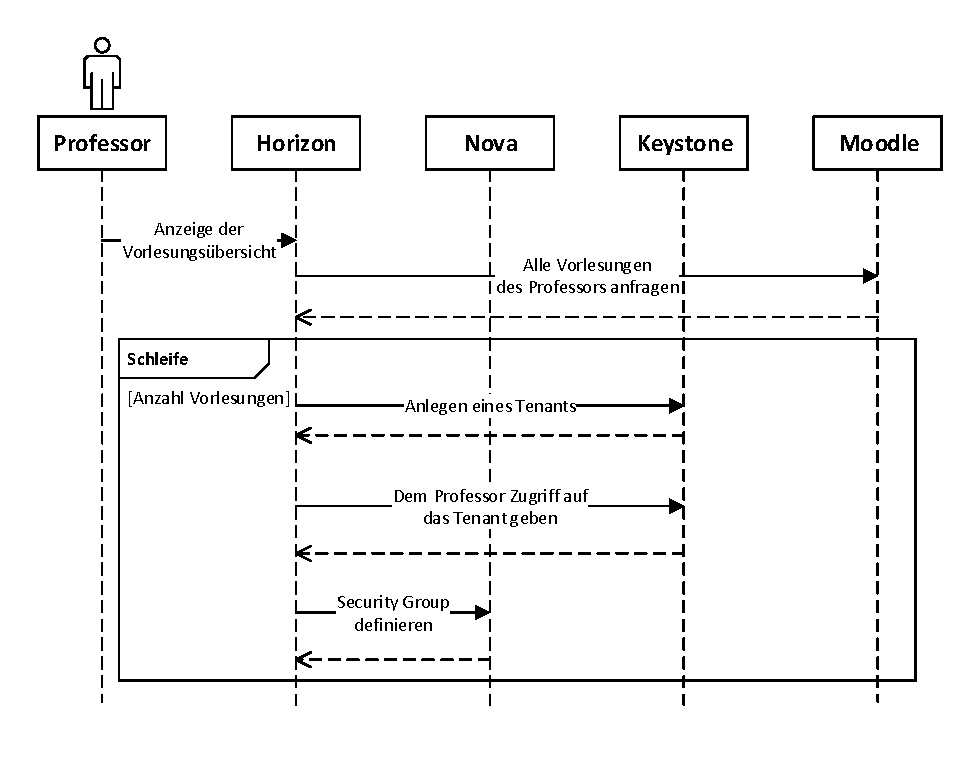
\includegraphics[scale=0.7]{img/createTenants.pdf}
\caption{Vorlesungen in der Cloud}
\label{createTenants}
\FloatBarrier
\end{figure}


\subsection{Starten von Instanzen}
Beim Starten der virtuellen Maschinen Instanzen einer Vorlesung 
(siehe Abbildung \ref{startInstances}) setzten wir voraus das für
die jeweiligen Vorlesungen bereits ein Tenant existiert. Wählen wir nun eine Vorlesung aus
(siehe hierzu auch Kapitel TODO), so wird zuerst eine Teilnehmerliste vom HTWG Moodle Server
angefragt. Dabei enthält die Teilnehmerliste die Namen und Email Adressen der Studenten.
Nun wird für jeden Teilnehmer eine Instanz gestartet. Die Instanz wird dabei für das jeweilige
Tenant gestartet und folgt einem vorgegebenen Namensschema. Das Schema ist eine Kombination
aus der Email Adresse des Teilnehmers und dem Namen des Tenants. Durch die eindeutige Namensvergabe
wird sichergestellt das nicht mehrere Instanzen für einen Studenten in einem Tenant gestartet
werden können.
Die Instanz wird dabei über Nova gestartet. Nach dem Starten der Instanz wird noch ein Blockgerät
über Cinder angelegt, welches daraufhin mit der jeweiligen Instanz verbunden wird. Dadurch können
Studenten ihre Daten ablegen.
Zuletzt wird dem Studenten eine Email mittels dem HTWG SMTP Server übermittelt, welche einen
Link für den Zugriff auf seine virtuelle Maschine über VNC enthält.

\begin{figure}[H]
	\centering
	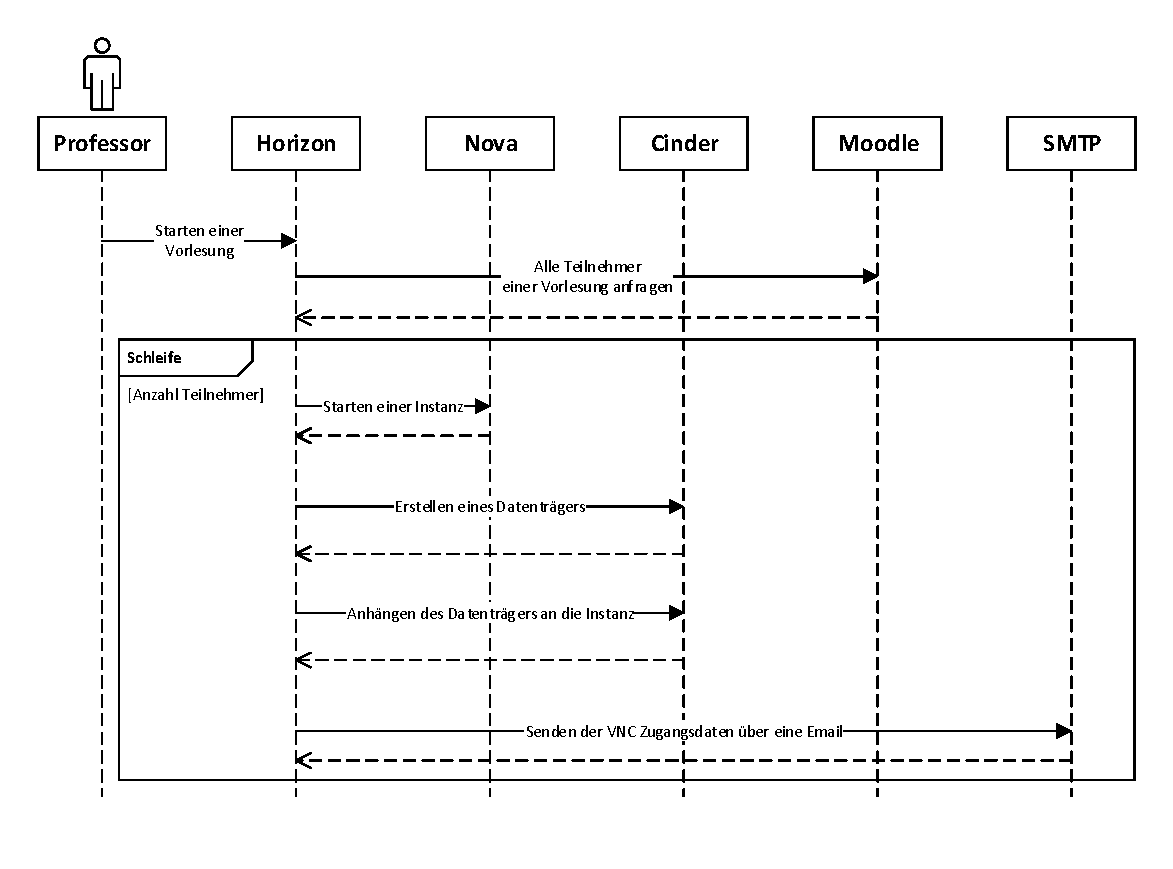
\includegraphics[scale=0.6]{img/startInstances.pdf}
\caption{Instanzen für eine Vorlesung starten}
\label{startInstances}
\FloatBarrier
\end{figure}

\subsection{Stoppen von Instanzen}
Das Stoppen der virtuellen Maschinen, welches unter Abbildung \ref{stopInstances} dargestellt ist,
soll hiermit auch erwähnt werden.
Beim Stoppen wird kein nicht zuerst eine Teilnehmerliste vom HTWG Moodle Server angefragt, wie
wir es noch beim Starten der Instanzen gesehen haben. Stattdessen wird über Nova eine Anfrage
gestellt um alle Instanzen des jeweiligen Tenants zu erhalten. Die so erhaltenen Instanzen werden
daraufhin gelöscht. Das selbe wird mit den Blockgeräten gemacht, welche beim starten einer
Instanz erstellt wurden. Für die Blockgeräte Verwaltung ist Cinder zuständig.

\begin{figure}[H]
	\centering
	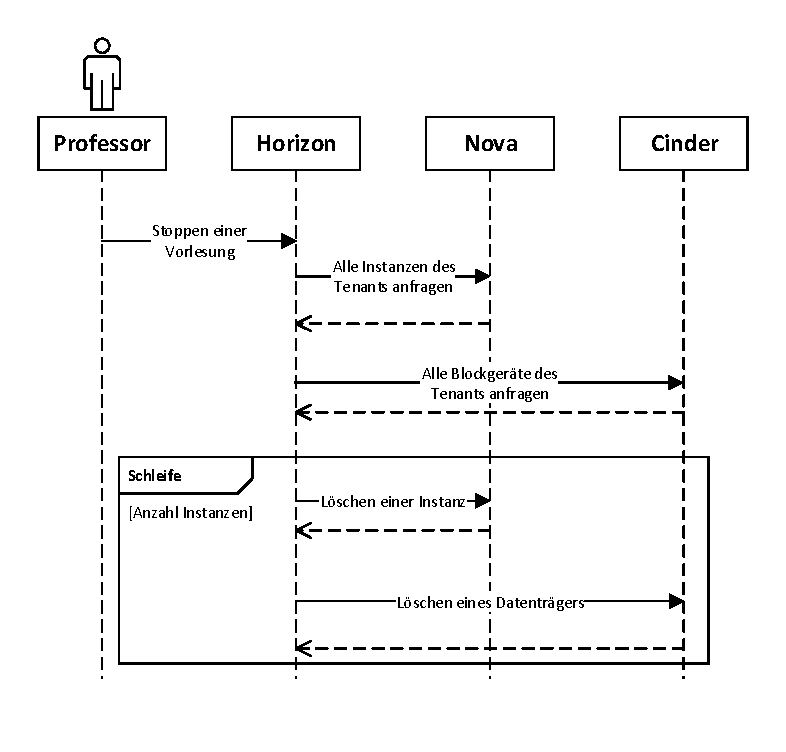
\includegraphics[scale=0.6]{img/stopInstances.pdf}
\caption{Instanzen einer Vorlesung stoppen}
\label{stopInstances}
\FloatBarrier
\end{figure}

\subsection{Aktualisieren einer Vorlesung}


\section{Dashboard}

Das unter dem Codenamen Horizon entwickelte webbasierte Dashboard dient der vereinfachten Verwaltung der OpenStack-Umgebung. Die Komponente wurde in der Programmiersprache Python implementiert und nutzt neben dem Django-Framework für Webapplikationen auch Apache 2.0 als Webserver. Gegenüber der Kommandozeilen-Variante besitzt das Dashboard zwar einen beschränkten Funktionsumfang, jedoch können die wichtigsten administrativen Verwaltungsaufgaben durchgeführt werden. Dazu zählen unter anderem:
\begin{itemize}
\item Integration von Images
\item Management der Instanzen
\item Verwaltung der Volumes
\item Einrichtung von Security Rules
\item Logs und Reports
\item VNC
\item etc.
\end{itemize}
Aufgrund des modularen Aufbaus von OpenStack kann das Dashboard individuell angepasst und erweitert werden. Die zugehörigen Schritte zur Anpassung des Frontends und Umsetzung einer funktionellen Erweiterung sind nachfolgend beschrieben.

\subsection{Anpassung von Horizon}

Zur Vereinheitlichung des Designs wurde das Dashboard an das HTWG-Design angepasst. Somit fügt sich die HTWG Lab Cloud nahtlos in das offizielle HTWG Design ein.

\begin{figure}[htbp]
\centering
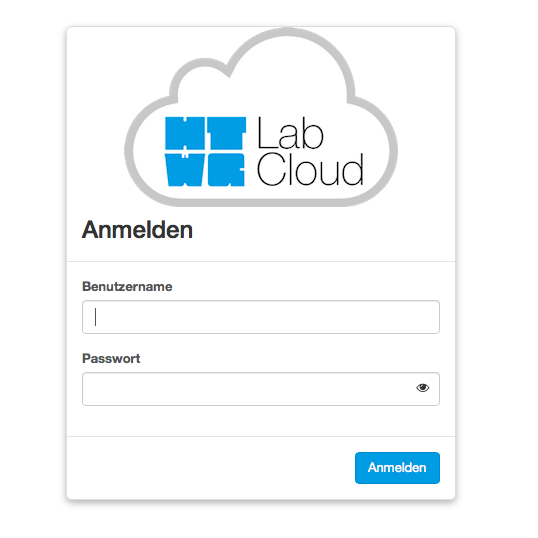
\includegraphics[scale=0.4]{img/dashboard-login.png}
\caption{HTWG Lab Cloud Dashboard Login}
\label{dashboard-login}
\end{figure}

Der Anmeldebildschirm zeigt das HTWG Lab Cloud Logo (vgl. \autoref{dashboard-login}).
Die Blautöne entsprechen denen der HTWG.
Ebenso wurden die anderen Ansichten im Dashboard alle an das HTWG Design angepasst (vgl. \autoref{dashboard-overview}).

\begin{figure}[htbp]
\centering
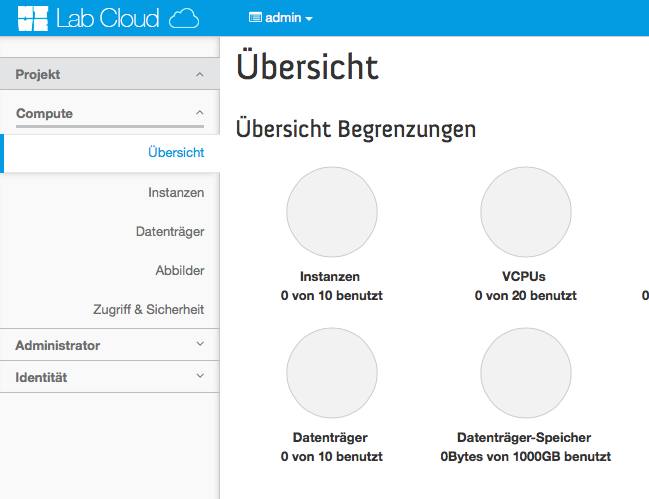
\includegraphics[scale=0.6]{img/dashboard-overview.png}
\caption{Übersichtsseite HTWG Lab Cloud Dashboard}
\label{dashboard-overview}
\end{figure}

Realisiert wurde die Anpassung mittels SCSS\footnote{Sass-CSS, eine erweiterte CSS Sprache.} und dem Theme-Mechanismus von Horizon.
Dabei müssen lediglich eine Datei und der \code{lab-cloud} Theme-Ordner in das Horizon Verzeichnis kopiert werden.
Ein anschließendes \code{python manage.py collectstatic --noinput --clear && python manage.py compress --force && sudo service apache2 restart} im Horizon Ordner kompiliert die Themes und starten den Webserver neu.

\subsection{Erweiterung von Horizon}

\begin{description}
\item[Dashboard und Panels: ]
\item[TabGroups und Tabs: ]
\item[DataTables: ] 
\item[Workflows: ] 
\item[Actions: ] 
\item[URLs: ] 
\item[Views: ] 
\end{description}

\section{OpenStack LDAP-Authentifizierung}\label{ldap_auth1}

\section{Anbindung an Moodle}


\section{Fernzugriff (VNC)}

Meist wird in OpenStack Umgebungen lediglich von Instanzen ohne graphische Oberfläche ausgegangen, auf denen beliebige Serveranwendungen laufen. 
Der dadurch oft genannte SSH-Zugang ist dafür vollkommen ausreichend.
Die HTWG Lab Cloud stellt jedoch eher eine \emph{Virtual Desktop Infrastructure} bereit.
Benutzer, insbesondere von nicht-technischen Studiengängen erwarten die gewohnte graphische Desktopumgebung (z. B. Unity oder KDE) in dieser Cloud-Lösung.

Da VNC ein unsicheres Protokoll ist, sollte es stets durch einen gesicherten Tunnel hindurch verwendet werden.

Der OpenStack VNC Console Proxy bietet diese Funktionen an.
Um die URL für den VNC Server zu erhalten erfolgt der Aufruf \code{nova get-vnc-console server_id novnc}.
Schließlich ist für den Zugriff lediglich die URL mit dem Access-Token notwendig, welche der Benutzer per E-Mail nach Start seiner Instanz erhält.
Anschließend kann auf die Instanz über den Browser zugegriffen werden.
Mobile Browser werden unterstützt, jedoch benötigen manche Browser eine virtuelle Tastatur. 
Dies kann erreicht werden, in dem die \code{vnc_auto.html} Datei noch angepasst wird.
NoVNC bringt die Funktionalität grundsätzlich mit.

\section{Snapshots}

Das hier vorgestellte Basis-Image stellt lediglich die Grundfunktionalitäten bereit. 
Um maximalen Nutzen aus der HTWG Lab Cloud zu ziehen, ist es elementar das Image an die jeweilige Übung möglichst genau anzupassen.

Hierbei wurden die Boardmittel von OpenStack evaluiert.
Wie sich herausgestellt hat, bietet OpenStack mit der \emph{Snapshot} Funktionalität genau dieses Feature an.
Von einer erstellten Instanz kann jederzeit ein Snapshot angefertigt werden.
Dieser entspricht exakt einem neuen herkömmlichen Image.

Also kann ein Professor das Basis-Image in einer Instanz starten, an die Übungsstunde anpassen und über \emph{Snapshot} ein neues Image erstellen.
Anschließend wird das Image beim Start der Instanzen ausgewählt.

\section{Netzwerk}

Die Netzwerkstruktur basiert auf der \emph{FlatDHCP} Struktur von nova-network. 
Dabei werden drei Netzwerkadapter mit folgender Konfiguration verwendet:

\begin{itemize}
\item eth0: NAT Interface, welches den Internetzugriff bereitstellt. Auf diesem Adapter läuft auch ein DHCP Server.
\item eth1: Interface ohne DHCP und Internetzugriff. Wird als Management-Netzwerk bzw. internes Netzwerk verwendet, über das die einzelnen Instanzen miteinander kommunizieren können. Muss sich im Promiscous Modus befinden, damit die Netzwerkpakete korrekt weitergereicht werden. Bei Installation in einer Virtuellen Maschine ist dieser Adapter auf \emph{host-only} geschaltet.
\item eth2: Interface auf dem öffentliche IP-Adressen der Instanzen allokiert werden und das HTWG Lab Cloud Dashboard erreichbar ist. Bei Installation in einer Virtuellen Maschine ist dieser Adapter mit dem Modus \emph{bridged}  mit einem lokalen, öffentlich zugänglichen Adapter verbunden.
\end{itemize}

Zusätzlich wird automatisch eine Bridge erstellt welche die Instanzen (an den Adaptern vnetX) mit dem Adapter eth1 verbindet.
Bei Installation außerhalb einer Virtuellen Maschine, kann der Adapter eth2 und eth0 zusammengelegt werden. 
Diese Trennung ist lediglich in einer Virtuellen Maschine erforderlich, um von außerhalb auf die HTWG Lab Cloud bzw. die Instanzen zugreifen zu können.
Denn der Adapter eth2 stellt den Zugang von außerhalb über den bridged Modus zur Verfügung.
Des Weiteren muss auf dem Host noch mittels \code{iptables -t nat -A POSTROUTING -o eth0 -j MASQUERADE} Source-NAT aktiviert werden, sodass die Instanzen Internetzugriff haben.

\section{Compute Image}

Da die OpenStack Umgebung gewisse Anforderungen an das Instanz-Image stellt, wurde in diesem Projekt ein Basis-Image entwickelt. 
Dieses kann in der OpenStack Umgebung gestartet und vom Professor für die jeweilige Übung angepasst werden.
Grundsätzlich sind in OpenStack Windows XP, 7, 8 und Linux-basierte Betriebssysteme als Instanz konfigurierbar. 
Aus lizenzrechtlichen Gründen wurde die Entscheidung für das Linux-basierte Betriebssystem \emph{Ubuntu} getroffen. 
Prinzipiell lassen sich die hier durchgeführten Anpassungen auch auf Windows übertragen, wobei die konkrete Konfiguration abweicht.

Der Workflow, um ein Image anzupassen und nachfolgend Instanzen mit diesem den Studenten bereitzustellen ergibt sich wie folgt:

\begin{enumerate}
\item Starten des Basis-Images in einer Instanz durch den Professor.
\item Installation von Programmen, Konfiguration der Instanz und andere Anpassungen.
\item Erstellen eines Snapshots, um die Änderungen festzuhalten. Dies erzeugt ein neues Image.
\item Starten der einzelnen Instanzen für die Studenten. Dabei wird die Instanz automatisch an den Student angepasst, sodass nur dieser Zugriff mittels seiner im LDAP hinterlegten Zugangsdaten hat.
\end{enumerate}

Im Folgenden wird auf die einzelnen Komponenten, die im Zuge dieser Projektarbeit erarbeitet wurden, eingegangen. 

\subsection{Details}

Als Betriebssystem wurde Ubuntu 14.04 Desktop LTS ausgewählt. 
Dieses ist zwar nicht die neuste Ubuntu-Version, bietet jedoch aufgrund des \emph{Long Term Support} Updates und relevante Sicherheitsfixes für 5 Jahre. 
Somit ist gewährleistet, dass das Basis-Image bis 2019 mit relevanten Updates versorgt wird. 
Insbesondere unter Betrachtung des Support-Aufwands durch das HTWG-Rechenzentrums soll so eine lange Laufzeit gewährleistet werden.

Aufgrund der Dateigröße ($> 5$ GB) kann das Image nicht in Git eingecheckt werden und wird über Dropbox \cite{dropboxImage} bereitgestellt. Das Image kann auch direkt bei den Autoren der Projektarbeit angefordert werden.

Da das Basis-Image noch keine personenbezogenen Daten enthält, wird ein Standard-Account mit \code{sudo} Rechten bereitgestellt:

\begin{itemize}
\item \emph{Benutzer:} ubuntu (Vollständiger Name: HTWG Lab Cloud)
\item \emph{Passwort:} ubuntu
\end{itemize}

Das von uns bereitgestellte Image enthält bereits einige Standardprogramme:

\begin{itemize}
\item Unity als Desktop-Manager
\item Dropbox
\item git
\item openssh-server
\item vim
\item OpenOffice
\item Firefox
\item und weitere Office-Applikationen
\end{itemize}

Auf andere Cloudspeicher-Anbieter musste verzichtet werden, da Google Drive und Windows OneDrive Linux nicht nativ unterstützen.

\subsection{Cloud-Kompatibilität}

OpenStack stellt gewisse Anforderungen an die Gast-Betriebssysteme, die sich im OpenStack Handbuch \cite{osImageRequirement} nachschlagen lassen. 
Die initiale Konfiguration des Basis-Images wurde aus Performance-Gründen in VirtualBox durchgeführt.
Durch Installation einiger Pakete und Anpassung von Konfigurationsdateien, wurde das Ubuntu Image OpenStack kompatibel gemacht:

\begin{itemize}
\item Installation von \code{cloud-init}, \code{cloud-utils} und \code{cloud-initramfs-growroot} *
\item Anpassen der Kernel-Boot-Parameter in der Datei \code{/etc/default/grub}. Dort wurde der Parameter \code{console=tty,ttyS0} ergänzt. Ein anschließendes \code{update-grub} aktualisert den Grub-Bootloader. Diese Änderung aktiviert die Ausgabe der Log-Meldungen im Horizon-Dashboard.
\item Anpassen von \code{cloud.cfg} des Pakets \code{cloud-init}. Dieses deaktiviert standardmäßig den Passwort-Login des Images. Da sich Nutzer jedoch per LDAP bzw. mit dem Standardbenutzername anmelden können sollen, muss dies aktiviert werden. *
\end{itemize}

Die mit * gekennzeichneten Punkte werden von dem entworfenen Skript \code{cloud-init-script.sh} automatisch ausgeführt. 
Anschließend löscht sich das Skript und fährt das Betriebssystem herunter.
Da nach Ausführung des \code{cloud-init-script.sh} Skripts das Image in VirtualBox nicht mehr ohne weiteres gestartet werden kann, sollte das Skript am Ende der Konfiguration ausgeführt werden.

\subsection{Konvertierung von VirtualBox nach OpenStack}

Nachdem das Basis-Image konfiguriert und kompatibel zu OpenStack gemacht wurde muss das Image noch in ein Format gewandelt werden, das OpenStack versteht.
Das entwickelte Skript \code{image-virtualbox-to-openstack.sh} führt diese Umwandlung aus. 
Die Benutzung erfolgt mit folgendem Aufruf: \code{./image-virtualbox-to-openstack.sh <Pfad zum gewünschten VirtualBox Image Snapshot>}.
Im Wesentlichen wird dabei mittels \code{VBoxManage} das Image in ein \code{raw} Format gewandelt und anschließend mit \code{qemu-img} nach \code{qcow2} überführt.

\subsection{LDAP-Authentifizierung}\label{ldap_auth2}

Studenten sollen sich mit ihren gewohnten HTWG Zugangsdaten bei den Instanzen anmelden können. 
Deshalb wird auf den LDAP-Server der HTWG zugegriffen, um den Benutzer beim Login in das Betriebssystem zu authentisieren. 
Da lediglich lesender Zugriff auf den LDAP-Server notwendig ist, sind keine speziellen Rechte erforderlich, um  mit dem LDAP-Server zu kommunizieren (insbesondere ist kein \emph{Bind DN} erforderlich).

Der HTWG LDAP-Server ist unter \url{ldap.htwg-konstanz.de} über die LDAP-Version 3 im Hochschulnetz erreichbar. 
Um auf das Wurzelverzeichnis zugreifen zu können, muss der \emph{Base DN} \code{dc=fh-konstanz,dc=de} gewählt werden. 
Einzelne Benutzer lassen sich mit dem DN \code{ou=users,dc=fh-konstanz,dc=de} auslesen, wobei die ungefilterte Anzeige auf 50 Benutzer begrenzt ist. 

Für das Projekt sind die Attribute

\begin{itemize}
\item uid: Benutzername
\item uidNumber: Benutzernummer
\item gidNumber: Gruppennummer
\item homeDirectory: Pfad zum home-Laufwerk
\item loginShell: Die für den Login genutzte Shell
\end{itemize}

relevant. Alle Attribute finden sich im HTWG LDAP-Server wieder und müssen somit nicht explizit gemappt werden. 
Eine Besonderheit besteht darin, dass die Attribute uidNumber, gidNumber, homeDirectory und loginShell bereits mit HTWG-spezifischen Werten belegt sind. 
So ist z. B. homeDirectory mit \enquote{/rzhome/username} vorbelegt.
Diese Werte lassen sich nicht für dieses Projekt verwenden.
Um trotzdem mit der HTWG interoperabel zu bleiben, werden diese Einträge beim Auslesen mittels \code{nss_override_attribute_value} überschrieben. 
Dabei werden jedoch im LDAP-Server \emph{keine} Einträge verändert, lediglich dem lokalen System erscheint der Eintrag als modifiziert.

Die Benutzer- und Gruppennummer wird auf fix auf 2000 gesetzt.
Damit ist genügend Raum für weitere lokale Benutzer, die eventuell von Programmen angelegt werden und automatisch bei 1001 starten.
Benutzer werden die Gruppen <username>, adm, cdrom, sudo, dip, plugdev, lpadmin, sambashare zugewiesen. 
Diese entsprechen den Ubuntu Standardgruppen eines neuen Benutzers.

\begin{figure}[htbp]
\centering
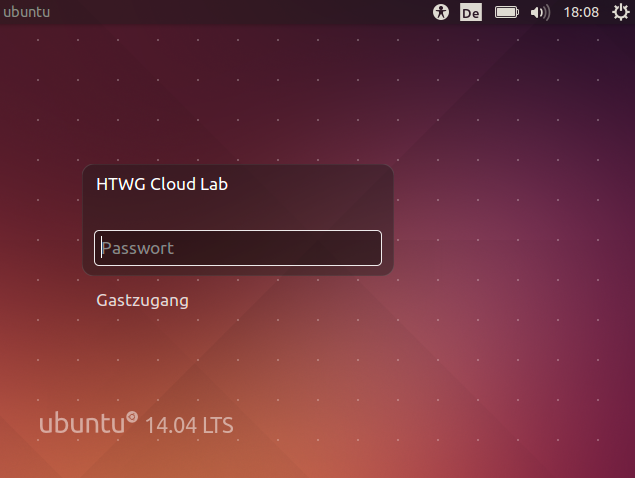
\includegraphics[scale=0.6]{img/lightdm.png}
\caption{Grafischer Login mit LightDM}
\label{lightdm}
\end{figure}

Betriebssystemseitig müssen die Pakete \code{ldap-auth-client} und \code{nscd} installiert werden. 
Die Authentifizierung wird mit dem Pluggable Authentication Modules (PAM) Framework realisiert. 
Mit dessen Hilfe lässt sich die Authentifizierung vom üblichen System abkoppeln und in ein LDAP-Modul auslagern.

Sicherheitsrelevant ist außerdem, dass eine einzelne Instanz nur von einem Benutzer erreichbar ist. 
Andernfalls besteht Gefahr, dass sich andere Nutzer auf der Instanz mit ihren Zugangsdaten anmelden und mittels \code{sudo} Adminrechte erlangen.
Danach wäre der Zugriff auf eventuell sensible private Daten (Cloudspeicher, HTWG home-Laufwerk, etc.) möglich.

Zur Verhinderung dieses Szenarios wird die LDAP-Authentifizierung durch die Zeile  \code{nss_base_passwd uid=<username>} auf den jeweiligen Benutzer beschränkt.
Somit wird die Suche für das Passwort eines Benutzer im LDAP-Verzeichnis gefiltert.

Schlussendlich sollen sich Benutzer über die gewohnte graphische Oberfläche (vgl. \autoref{lightdm}) am System anmelden können.
Hierzu muss der Login-Manager \emph{LightDM} konfiguriert werden und die Eingabe eines beliebigen Benutzernamens erlauben (ggü. dem Standard, der nur lokale Benutzer aus einer Liste zur Auswahl anbietet).
Dieses Ziel wurde erreicht, in dem die \code{SeatDefaults} in der entsprechenden Konfigurationsdatei angepasst wurden.

Da diese Installationen der Pakete normalerweise einen interaktiven Dialog erfordern, musste ein Weg gefunden werden, um dies automatisiert ausführen zu lassen.
Hier war der Befehl \code{DEBIAN_FRONTEND=noninteractive apt-get -y -q install ..} hilfreich. 
Dadurch werden bei interaktiven Dialogen die Standardwerte angenommen und alles weitere ohne Nachfrage installiert. 
Die anschließende manuelle Änderung der Konfigurationsdateien über ein Skript stellt die korrekten Einstellungen sicher.

Alle vorhergehenden Konfigurationen werden in den folgenden Dateien durchgeführt. 
Die genauen Details finden sich in den Readme und Skript Dateien bei den Projektquellen.

\begin{itemize}
\item \code{/etc/nsswitch.conf}: LDAP als PAM Authentifizierungsmodul
\item \code{/etc/ldap.conf}: LDAP Konfiguration inkl. Attributmapping und -überschreiben
\item \code{/etc/pam.d/common-session}: Erstellen des lokalen home Verzeichnisses beim erstmaligen Login
\item \code{/etc/security/group.conf}: Zuweisung von lokalen Systemgruppen an LDAP Benutzer
\item \code{/etc/pam.d/common-auth}: Hinzufügen des PAM Gruppenmoduls
\item \code{/etc/group}: Definition der Systemgruppen für den jeweiligen LDAP-Benutzer
\item \code{/etc/lightdm/lightdm.conf}: LDAP Login über den graphischen Login-Manager ermöglichen
\end{itemize}

\subsection{HTWG home-Laufwerk}

Eine weitere Dienstleistung besteht darin, dem Benutzer sein gewohntes HTWG home-Laufwerk zur Verfügung zu stellen, um einen nahtlosen Wechsel zwischen OpenStack Instanz und lokalen Rechenzentrum-PCs sicherzustellen.

Das jeweilige home-Laufwerk unter \code{smb://homedrive.htwg-konstanz.de/home} erfordert eine Authentisierung des Nutzers gegenüber dem HTWG-Server. 
Jedoch soll aus Bequemlichkeitsgründen eine Single-Sign-On Lösung implementiert werden.
Der zentrale und einzige Login soll somit der Anmeldevorgang am Betriebssystem sein.

Als ideale Lösung stellt sich ein weiteres PAM-Modul heraus. \code{libpam_mount} bietet die gewünschte Funktionalität. 
Über zwei XML-Konfigurationsdateien wird das home-Laufwerk als \enquote{home-drive} unter \code{/media/home-drive} eingebunden.
Dadurch erscheint das Verzeichnis in der Seitenleiste des Nautilus Dateimanagers und ist komfortabel erreichbar.

\subsection{Block-Storage lab-drive}

OpenStack Instanzen können jederzeit neu gestartet oder erstellt werden.
Dies stellt die Verwaltung von benutzerspezifischen Dateien vor das Problem, auch über die Lebenszeit einer Instanz hinaus Daten speichern zu können. 

Die Block-Storage Komponente \emph{Cinder} bietet die Möglichkeit ein Stück Speicher mit Blockadressierung einer Instanz bereitzustellen. 
Dabei ist die Lebensdauer unabhängig von der Instanz. 
Dies erlaubt es, pro Übung eine neue Instanz zu starten mit jeweilig neuem Image, ohne wichtige Daten zu verlieren.

Zwar könnte grundsätzlich das home-Laufwerk der HTWG diese Stellung einnehmen, stellt aber aufgrund der sehr eingeschränkten Speicherkapazität keine zufriedenstellende Lösung dar.
Deshalb wird pro Instanz ein variabel großes Cinder-Laufwerk \enquote{lab-drive} erstellt und unter \code{/dev/vdb} angebunden.
Eine Herausforderung stellt die Hotplug-Fähigkeit dar. 
Das Laufwerk könnte zu jeder Zeit an die Instanz an- und abgeschlossen werden.
Des Weiteren muss beim ersten Anbinden das Laufwerk als ext4 formatiert werden.

Die Linux Systemdienste \code{mount mit fstab} und \code{udev} bieten die nötige Infrastruktur zur Realisierung.
Nachfolgen ist der Ablauf beschrieben, wie mit dem Laufwerk umgegangen wird bzw. die Tools installiert und konfiguriert werden.

\begin{itemize}
\item Einmaliges Erstellen des Mountpunktes \code{/media/lab-drive}.
\item Eintrag mit Mount-Informationen in \code{/etc/fstab} erstellen.
\item Ablages eines Skripts unter \code{/usr/local/bin/mount-lab-drive.sh}, welches das Mounten und Formatieren des Laufwerks übernimmt.
\item udev Regeldatei erstellen, die bei Änderungen im Linux Subsystem \code{block} das Mount-Skript aufruft.
\end{itemize}

Ebenso wie das home-Laufwerk erscheint das lab-drive in der Seitenleiste des Nautilus Dateimanagers.

\subsection{Installationsskript  für Benutzerkonfiguration}

Um die einzelnen Instanzen beim Erstellen auf einen Studenten anzupassen, muss das Image pro Student individuell verändert werden. 
Das \code{cloud-init} Paket bietet die Möglichkeit mittels dem Parameter \code{user-data} ein Skript beim Starten mitzugeben. 

Zur Installation der vorhergehend genannten Funktionen (LDAP-Authentifizierung etc.) wird ein generisches Skript generiert, welches nur noch minimal pro Student angepasst werden muss.
Dieses Skript \code{setup-instance.sh} wird durch ein Makefile erstellt, in dem alle \code{install.sh} Skripte der einzelnen Features aneinander gehängt und durch einen Header und Footer Teil ergänzt werden.
Im Header-Skript wird geprüft, ob root Rechte vorliegen und die \code{USER} Variable gesetzt wurde und \code{apt-get} aktualisiert. 
Der Footer ist dafür zuständig, nach dem Ausführen aller Teilskripte den Rechner neuzustarten.
Die \code{USER} Variable muss vor dem Ausführen durch den tatsächlichen Rechenzentrum Benutzernamen des Studenten ersetzt werden.
Im Dashboard wird mittels Python das Skript angepasst und als \code{user-data} Parameter gesetzt.

\section{Probleme bei der Implementierung}

Da OpenStack rasant weiter entwickelt wird, bleibt an einigen Stellen die Dokumentation auf der Strecke bzw. ist veraltet. 
Herauszufinden, wie die Dienste konfiguriert werden müssen war mit oftmals stundenlangen Recherchen verbunden.
Auch die Linux Module PAM mit LDAP sind sehr lückenhaft und veraltet dokumentiert.
Dies hat unweigerlich zu unzähligen Trial and Error Sitzungen geführt.
Meist resultiert die Lösung in nur wenigen Zeilen Code, diese jedoch mangels Dokumentation zu erstellen hat die Geschwindigkeit der Entwicklung stark gebremst.



WEITERES VON DEN ANDEREN SECTIONS


Die Netzwerkfunktionalität von OpenStack ist einerseits extrem flexibel, zugleich aber auch extrem kompliziert und nur schwer zu durchdringen.
Eine lauffähige Netzwerkumgebung aufzusetzen, erforderte ebenfalls großen Aufwand.

Ein weiteres Problem bestand in der Erstellung des Basis-Image aufgrund von Performance Problemen.
Auf einem handelsüblichen Notebook eine Virtuelle Maschine mit DevStack zu starten und in dieser dann nochmals ein komplettes Betriebssystem wie Ubuntu zu virtualisieren, zeigte der Hardware die Grenzen auf.
Deshalb musste zuerst ein VirtualBox Image konfiguriert und Skripte zur Umwandlung nach OpenStack entwickelt werden.

Insgesamt lässt sich mit einem so komplexen System wie OpenStack kein schneller Program-Compile-Execute Zyklus durchführen.

\section{Bekannte Bugs}

\begin{itemize}
\item Der LDAP-Login am Image muss zweimal durchgeführt werden. Hier liegt ein Bug seitens des LightDM Login-Managers vor.
\end{itemize}